%=======================================================================
\section{Part A: The Training Data}
\label{sec:data}

\subsection{Overview}

Each protease model is trained on confirmed cleavage windows. Three
sources contribute: the MEROPS \texttt{Substrate\_search} table \cit{8},
which lists for each recorded cleavage the eight residues around the
scissile bond; the proteomic identification of cleavage sites (PICS) data of
Eckhard et al.\ \cit{4} for MMP-2, MMP-8, MMP-9 and MMP-14; and the elastin
digestion data of Yang et al.\ \cit{5} for LasB. In PICS, an MMP is incubated
with peptide libraries derived from a human proteome digested with trypsin or
GluC, and cleavage products are identified by LC-MS/MS at a false-discovery
rate of 1\%; the non-primed residues $\pos{4}$--$\pos{1}$ are recovered by
locating each identified peptide in its source protein sequence. The Yang et
al.\ study identified peptides released from bovine elastin by pseudolysin by
mass spectrometry, and both termini of each released peptide are cleavage
sites.

\subsection{Assumptions}

\begin{assump}
\begin{itemize}[leftmargin=*,noitemsep]
\item \textbf{Confirmed windows are correct positives.} Windows are taken as
  recorded in the sources. The MEROPS table mixes physiological and synthetic
  substrates \FLAG.
\item \textbf{Negatives are unlabelled, not confirmed.} No window is known
  to be uncleaved; random background windows are assumed to be negatives.
  The resulting label noise is bounded in Part~\ref{sec:eval} but its
  magnitude is unknown \FLAG.
\item \textbf{Sources are pooled without correction for source bias.} PICS
  libraries are generated with trypsin or GluC, which constrains composition
  at peptide ends and may leak into primed positions of short peptides
  \FLAG.
\item \textbf{The LasB set is dominated by one protein.} $97$ of $128$
  positives ($76\%$) are windows from bovine elastin \CONF.
\item \textbf{The faecal group is heterogeneous.} It pools three
  unrelated digestive proteases (bovine trypsin~1, human chymotrypsin~B,
  porcine elastase-1) \CONF; its windows are capped at $5{,}000$ of $18{,}251$.
\end{itemize}
\end{assump}

\subsection{Sources and extraction}

MEROPS windows are read from columns $5$--$12$ of the substrate table
(three-letter code for $\pos{4}$ to $\prm{4}$), keyed by the peptidase
identifier in column~2. The Eckhard windows were extracted once from the
supplementary tables and archived; all peptides in the eight source sheets
used carry an N-terminal label ($3{,}536$ thioacyl at $+89.01$~Da and $815$ at
$+29.04$~Da, the latter not defined in the source legend) \CONF. The Yang et
al.\ Supplementary Table~S1 was re-extracted directly from the supplementary
PDF: all $75$ peptide rows were recovered, and for each row the peptide sits at
its stated position in the UniProt sequence of bovine tropoelastin (P04985)
and both flanking residues match, in all $75$ rows \CONF. The $\pos{4}$--$\prm{4}$
window is then read from that sequence around both termini of each peptide.
Rebuilding the MEROPS and Eckhard positive sets from the raw files reproduces
the counts obtained by the earlier implementation exactly \CONF.

\begin{center}
\small\renewcommand{\arraystretch}{1.25}
\begin{tabular}{@{}lrrrr@{}}\toprule
Protease & MEROPS & Eckhard 2016 & Yang 2015 & Total \\\midrule
MMP-2 & 2{,}318 & 501 & 0 & 2{,}819 \\
MMP-8 & 96 & 602 & 0 & 698 \\
MMP-9 & 341 & 442 & 0 & 783 \\
MMP-14 & 129 & 588 & 0 & 717 \\
Neutrophil elastase & 327 & 0 & 0 & 327 \\
LasB & 31 & 0 & 97 & 128 \\
Faecal serine proteases & 5{,}000 & 0 & 0 & 5{,}000 \\
\bottomrule\end{tabular}

\end{center}

The table lists positive windows per protease and source after removal of
duplicate windows; a window reported by several sources is counted once, under
the first.

\subsection{Negative sets}

For a target $t$ with $n_t$ positives the training set contains
$N=3n_t$ negatives. With $K-1=6$ competitor proteases, a quota
$q=\lfloor N/2/(K-1)\rfloor$ of windows is drawn without replacement from each
competitor's positives, excluding any window that is a positive of $t$. The
remaining negatives are random background windows whose residues are drawn
independently from the UniProtKB/Swiss-Prot amino-acid composition (release
2026\_03) \cit{10}, again excluding known positives. For MMP-9, $N=2{,}349$:
$195$ windows from each of five competitors, $121$ from LasB (its entire
eligible pool), and $1{,}253$ background windows. Construction is seeded and
reproducible. Two alternatives are evaluated in Part~\ref{sec:eval}:
background-only negatives, and the design of the earlier implementation,
composition-shuffled positives plus background.

\subsection{Near-duplicate structure}

Sequence data of this kind contain families of near-identical windows
(collagen and elastin repeats, overlapping peptides from one protein, the same
site reported by two sources). If such windows are divided between training and
test folds, a model can score well by recalling a neighbour. A graph is
therefore defined on all training windows in which two windows are adjacent
when their Hamming distance is at most $2$ (at least $6$ of $8$ residues
identical), and its connected components are termed clusters. The fraction of
each positive set with a near-duplicate ranges from $2\%$ (NE) to $28\%$
(LasB); MMP-9 contains a single cluster of $86$ windows \CONF.

\begin{figure}[H]
  \centering
  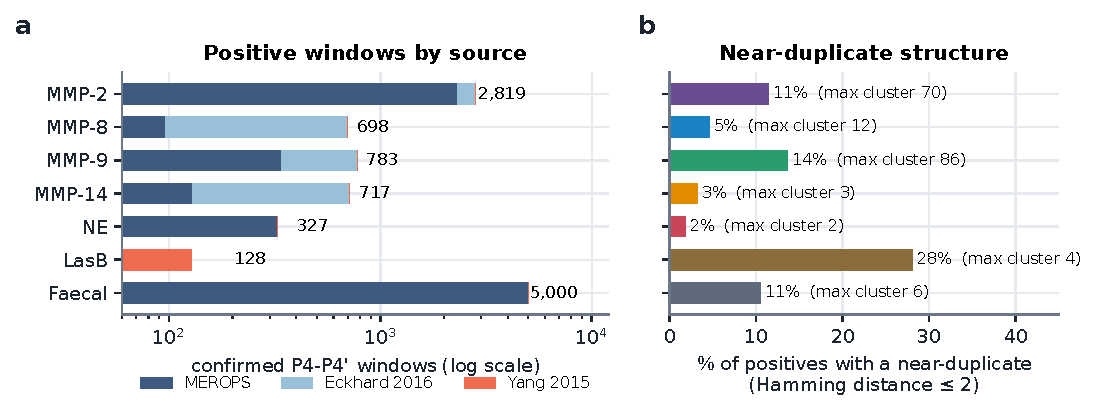
\includegraphics[width=\textwidth]{../figures/F02_data_composition.pdf}
  \caption{\textbf{A:} positive windows per protease by source (log scale).
    \textbf{B:} fraction of positives that have at least one near-duplicate
    (Hamming distance $\le2$) and the size of the largest cluster.}
  \label{fig:data}
\end{figure}

\subsection{Similarity between proteases}

Exact window overlap between protease positive sets is small (maximum Jaccard
index $0.145$, between MMP-8 and MMP-9), and windows shared with the target are
removed from its negatives. The position-specific preferences nevertheless
overlap strongly among the MMPs: the PSSM log-odds vectors of MMP-2, MMP-8 and
MMP-14 correlate at $r=0.73$--$0.82$, and MMP-9 correlates at $0.56$--$0.63$ with
each. NE is essentially uncorrelated with the MMPs and correlates with the
faecal group at $0.46$, both being serine proteases. This structure predicts
the selectivity results of Part~\ref{sec:eval}.

\begin{figure}[H]
  \centering
  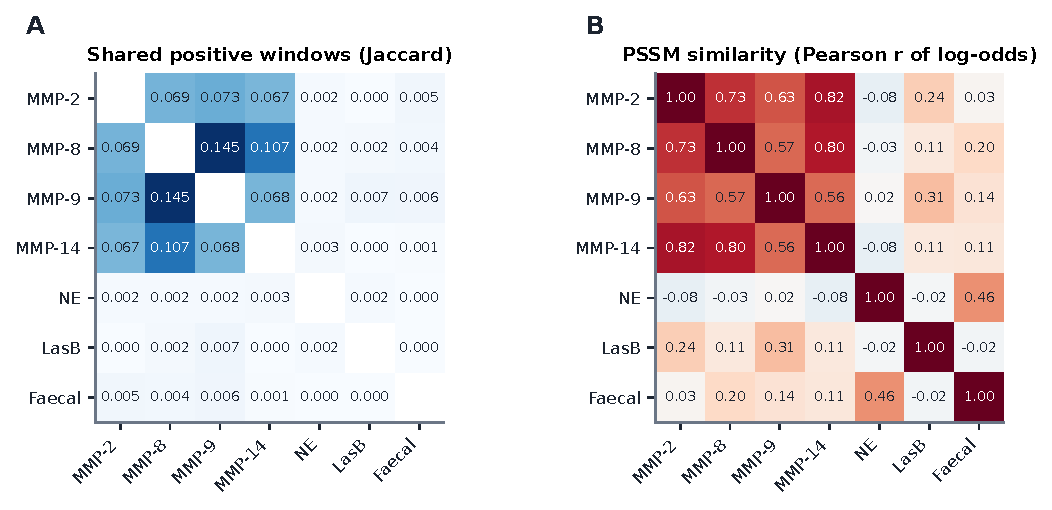
\includegraphics[width=\textwidth]{../figures/F04_protease_similarity.pdf}
  \caption{\textbf{A:} Jaccard index of exact positive windows.
    \textbf{B:} Pearson correlation of the $8\times20$ PSSM log-odds between
    protease pairs.}
  \label{fig:sim}
\end{figure}

\begin{figure}[H]
  \centering
  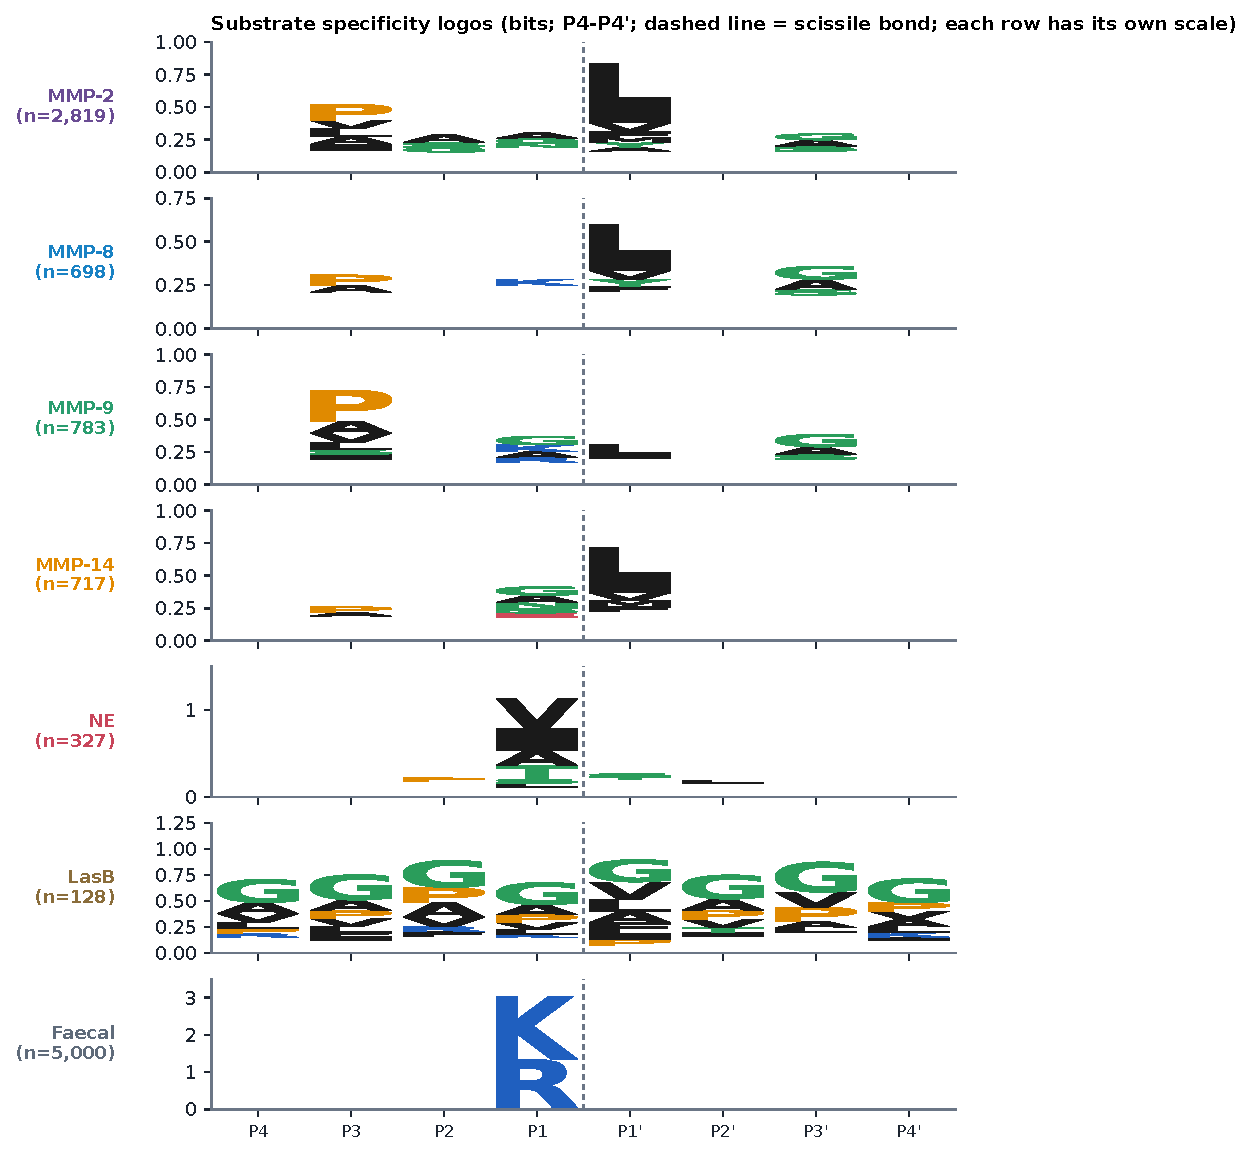
\includegraphics[width=0.86\textwidth]{../figures/F03_sequence_logos.pdf}
  \caption{Specificity logos computed from each model's PSSM (letter height is
    probability times information content; each row has its own vertical scale,
    since the MMPs carry under one bit per position while the faecal group
    exceeds three at $\pos{1}$). The MMPs share Pro at $\pos{3}$ and a
    hydrophobic residue at $\prm{1}$; NE prefers small aliphatic residues at
    $\pos{1}$; the faecal group is dominated by Lys/Arg at $\pos{1}$. The LasB
    logo is Gly-rich because $76\%$ of its positives derive from elastin.}
  \label{fig:logos}
\end{figure}

\subsection{Provenance checks and corrections}

Before the present models were built, each element of an earlier
implementation was tested with code (audit run at repository commit
\texttt{68e3dc2}; outputs retained in \texttt{results/legacy\_audit/}). The
findings, and the resulting action, are as follows.

\begin{center}
\footnotesize\renewcommand{\arraystretch}{1.2}
\begin{tabular}{@{}p{0.17\textwidth}p{0.47\textwidth}p{0.28\textwidth}@{}}
\toprule
Element & Finding & Action \\
\midrule
VHSE descriptor table & $35$ of $160$ values differed from the archived published table (several with opposite sign); glycine had been set to an all-zero reference vector, which is incorrect; descriptor labels contradicted the source definition (hydrophobic, steric, electronic); the citation named the wrong journal. Correction changed random-fold AUROC by $-0.006$ to $+0.012$. & Table regenerated from the archived file and unit-tested against it. \\
Swiss-Prot background & Two different frequency tables were in use (a residue frequency differed by up to $0.0049$). & One table from release 2026\_03. \\
Grouped cross-validation & Reported as $0.5$ for every protease: the groups were the labels positive, cross and background, so every held-out group contained one class and the function returned a fixed fallback. & Replaced by cluster-aware folds. \\
PSSM performance & Scored on the positives used to build the PSSM. In-sample versus out-of-fold AUROC: LasB $0.977$ versus $0.779$, NE $0.883$ versus $0.829$, MMP-8 $0.875$ versus $0.849$, MMP-9 $0.816$ versus $0.790$. & PSSM refit and scored out-of-fold in every fold. \\
Selectivity index & The ratio $p_t/\max p_j$ compared probabilities from models whose mean score on random windows ranged from $0.106$ to $0.328$; the median index of the top $1\%$ of MMP-9 candidates was $0.975$. & Percentile scale and margin (Part~\ref{sec:panel}). \\
LasB training data & $92$ positives were generated by a rule (every Ala$|$Ala, Val$|$Ala, Ala$|$Gly and Gly$|$Ala bond in a hard-coded elastin string) and attributed to a paper not held; $14$ more were typed by hand; four windows tagged as MEROPS were absent from the MEROPS file. None is a measured cleavage site. & Removed. LasB uses $31$ MEROPS windows and $97$ from Yang et al. \\
Elastin table & Typed by hand from the PDF; four of $75$ rows did not appear in the source. & Re-extracted from the PDF; $75$ of $75$ rows verified. \\
Kinetic table & The competing enzymes were labelled MMP-1 and MMP-2; the source gives MMP-13 and MMP-7. One measured non-substrate (C11) was omitted. & Re-extracted from the source table. \\
Report and code drift & Positive counts in the earlier report (MMP-14 $129$, MMP-8 $96$, MMP-9 $341$) no longer matched the data ($717$, $698$, $783$); a unit test asserted the incorrect glycine claim; oversampling was applied before cross-validation. & Report rewritten; test corrected; oversampling removed. \\
Model sprawl & Separate model files and scripts per experiment overwrote one another. & One model per protease. \\
\bottomrule
\end{tabular}
\end{center}

\subsection{Result}

The corrected data layer yields seven trainable proteases with
$2{,}819$ (MMP-2), $698$ (MMP-8), $783$ (MMP-9), $717$ (MMP-14), $327$ (NE),
$128$ (LasB) and $5{,}000$ (faecal group) confirmed windows. FAP is registered
but has only two confirmed windows in MEROPS and cannot be trained.
